\chapter{Instalación y uso de la \emph{app}}
Aquí se explican los primeros pasos y consideraciones a seguir para que todo aquel que esté interesado en utilizar la \textit{app}.
\section{Requisitos}
Esta aplicación sólo puede instalarse en dispositivos que tengan \textit{iOS 11.3} o posterior, ver figura~\ref{fig:target}. Además, los atajos de \textit{Siri} sólo funcionan a partir de \textit{iOS 12}, por lo tanto esta funcionalidad no estaría disponible para dispositivos que no estuviesen actualizados. Todos los dispositivos que soportan \textit{iOS 11}, también soportan \textit{iOS 12}.

\begin{figure}[tbp]
\centering
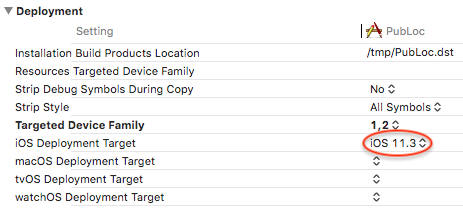
\includegraphics[scale=0.6]{figures/target.png}
\caption{Requisitos mínimos del sistema operativo.\label{fig:target}}
\end{figure}

\section{Instalación}
Todo aquel que quiera empezar a utilizar la aplicación sólo tiene que instalarla en su teléfono  \textit{iOS}. No está disponible en la \textit{Apple Store} todavía, así que tendría que obtener el ejecutable por otras fuentes e instalarlo manualmente \cite{noauthor_como_nodate}.

\section{Manual de usuario\label{apen:manual-usuario}}
En esta sección, se guiará al usuario a través de las diferentes pantallas de la aplicación, explicándole el contenido de las mismas y como debe interactuar con ellas.

\subsection{Pantallas principales}
Aquí hablaremos sobre las pantallas fundamentales de la aplicación, desde el inicio de sesión hasta el listado de ofertas.

\paragraph{Pantalla de inicio.} Se presenta la aplicación y se da la opción al usuario de iniciar sesión con \textit{Google} o de entrar directamente, ver figura~\ref{fig:inicio}.

\begin{figure}[tbp]
\centering
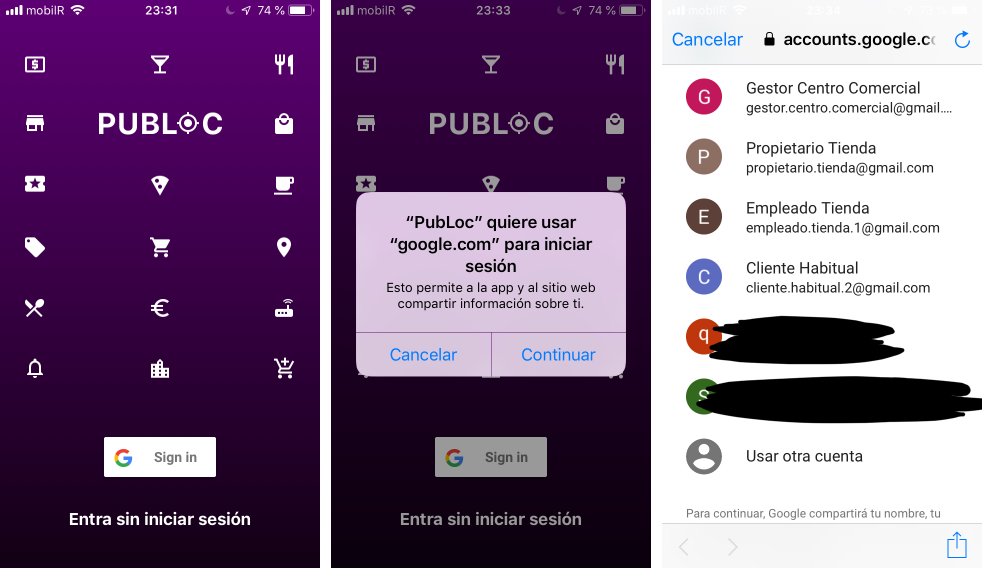
\includegraphics[scale=0.4]{figures/inicio.png}
\caption{Proceso de inicio y autenticación con \textit{Google}.\label{fig:inicio}}
\end{figure}

\paragraph{Centros comerciales.} La siguiente pantalla que se presenta es la misma independientemente de si el usuario está autenticado o no. Contiene una tabla en la que aparecen todos los centros comerciales que están dados de alta en \textit{Situm Dashboard}, en la parte inferior de la pantalla encontraremos un botón que permite al usuario ver su perfil y realizar algunos ajustes, ver subfigura~\ref{ref:centros-comerciales}.

\begin{figure}[tbp]
\centering
\subfigure{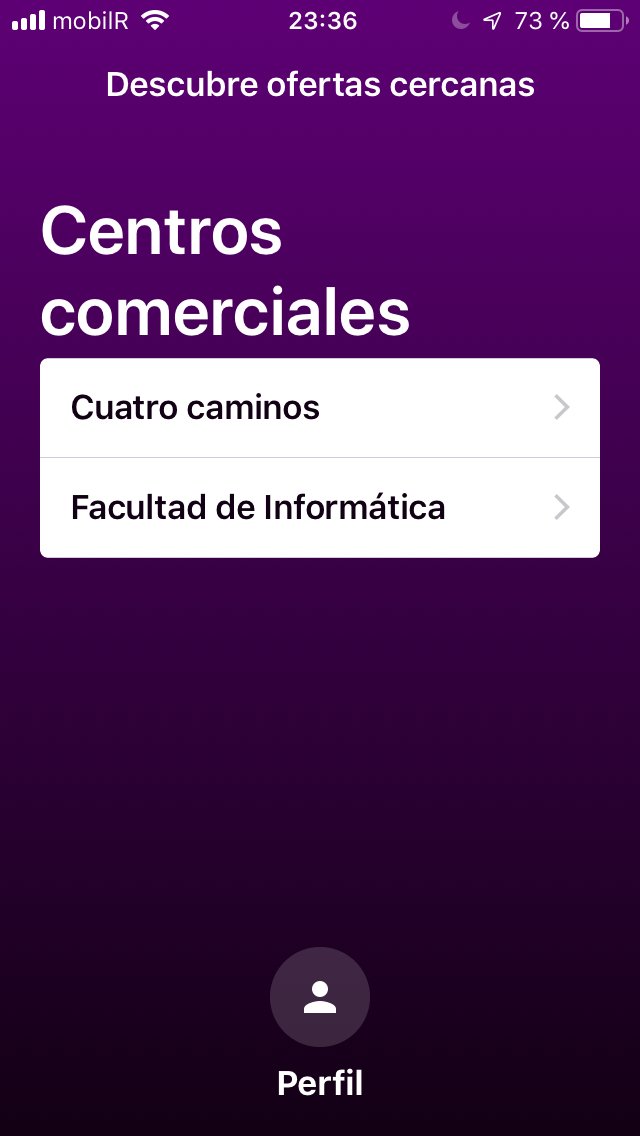
\includegraphics[scale=0.2]{figures/centros-comerciales.jpeg}\label{ref:centros-comerciales}}
\subfigure{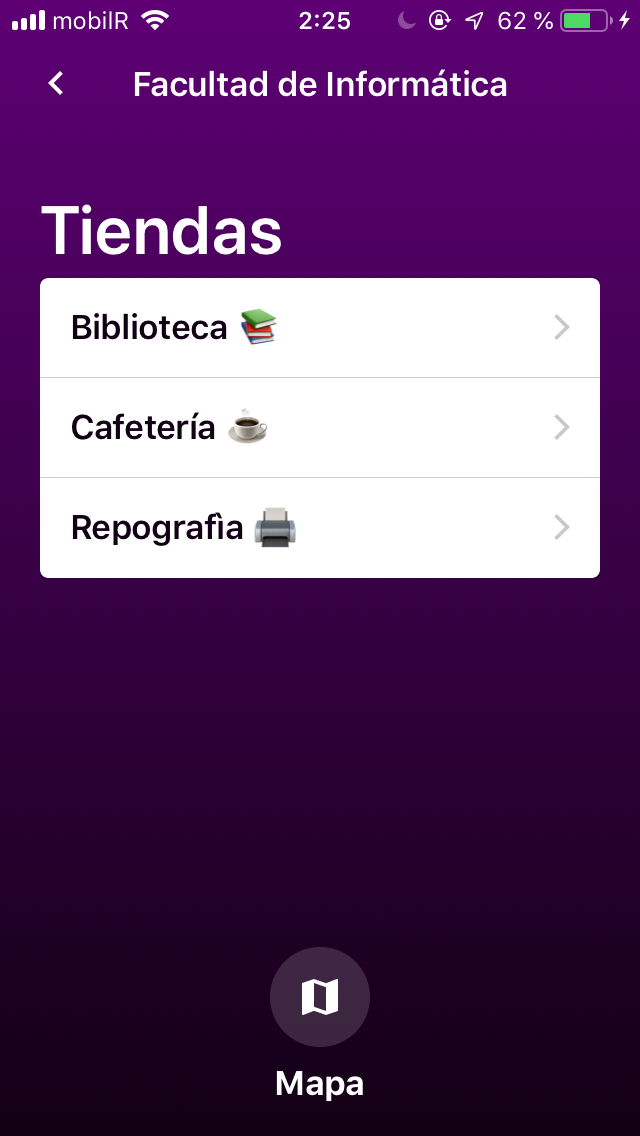
\includegraphics[scale=0.4]{figures/tiendas-map.jpeg}\label{ref:tiendas-map}}
\subfigure{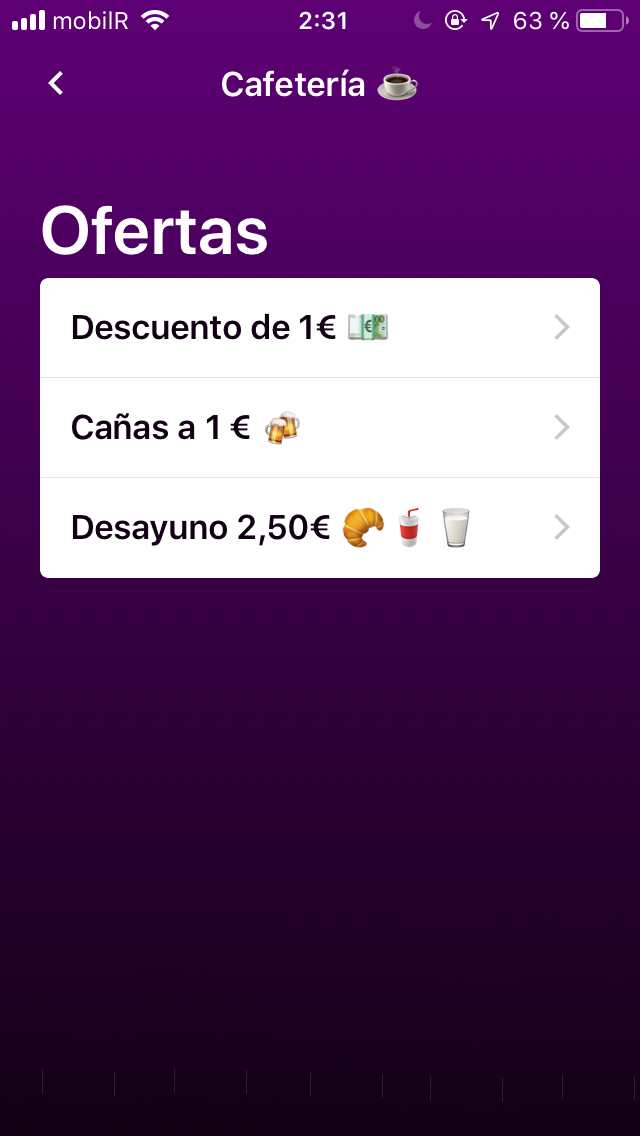
\includegraphics[scale=0.4]{figures/ofertas.jpeg}\label{ref:ofertas}}
\caption{Tablas: (a) Centros comerciales, (b) tiendas de un centro comercial y (c) ofertas de una tienda.}
\end{figure}

\paragraph{Tiendas.} Si el usuario selecciona un centro comercial entonces se mostrarán las tiendas que están dadas de alta en la plataforma. En esta pantalla también hay un botón que nos llevará a un mapa en el cual hemos cargado los planos del edificio, ver subfigura~\ref{ref:tiendas-map}.

\paragraph{Ofertas.} Y si finalmente el usuario selecciona una tienda, podrá ver las ofertas que ha dado de alta el propietario de la misma, ver subfigura~\ref{ref:ofertas}. Seleccionando una, se verá el detalle de la misma.

\subsection{Detalle de oferta}
Cuando seleccionamos una oferta concreta, se mostrará una pantalla con más información, ver subfigura~\ref{fig:detail}. Esta pantalla se merece una subsección para ella sola porque tiene muchos componentes.

\paragraph{Código \textit{QR}.} El cliente deberá mostrarlo al empleado de tienda para canjear la oferta, sólo aparecerá en caso de que el usuario esté autenticado. Si no, se mostrará un botón para que inicie sesión con \textit{Google} si así lo desea.

\paragraph{Descripción.} Breve texto descriptivo sobre la oferta.

\paragraph{Contador de ofertas restantes.} Aquí se mostrarán en tiempo real las ofertas que quedan disponibles.

\paragraph{Cuenta atrás.} Indica el tiempo que queda para que caduque la oferta.

\paragraph{Botones de \textit{like}/\textit{dislike}.} Así el usuario podrá indicar si no le interesa que se le notifique esa oferta dándole a \textit{like}. Pero si seleccionase \textit{dislike}, entonces la oferta quedaría archivada en el listado de ofertas favoritas que comentaremos más adelante. Al igual que el código \textit{QR}, estas funciones sólo estarán activadas en caso de que el usuario este autenticado, en caso contrario, los botones aparecerán, pero deshabilitados.

\paragraph{Ver en mapa.} Mostrará la situación de la oferta en el plano del edificio, ver subfigura~\ref{fig:map-detail}.

\begin{figure}[tbp]
\centering
\subfigure{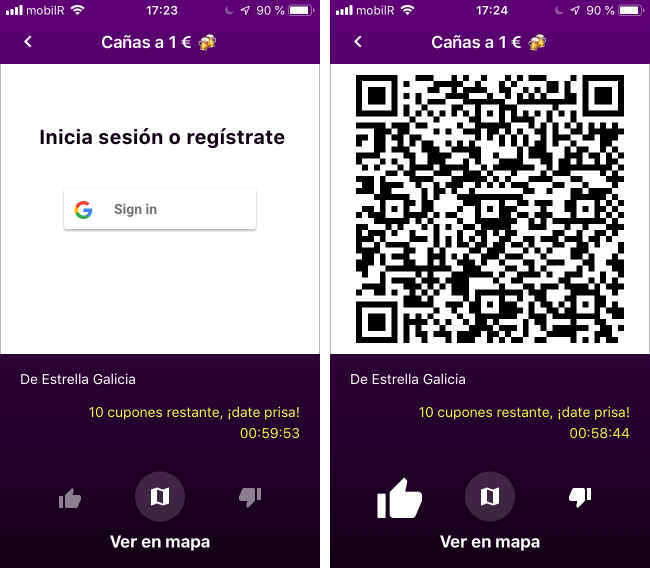
\includegraphics[scale=0.4]{figures/detail.png}\label{fig:detail}}
\subfigure{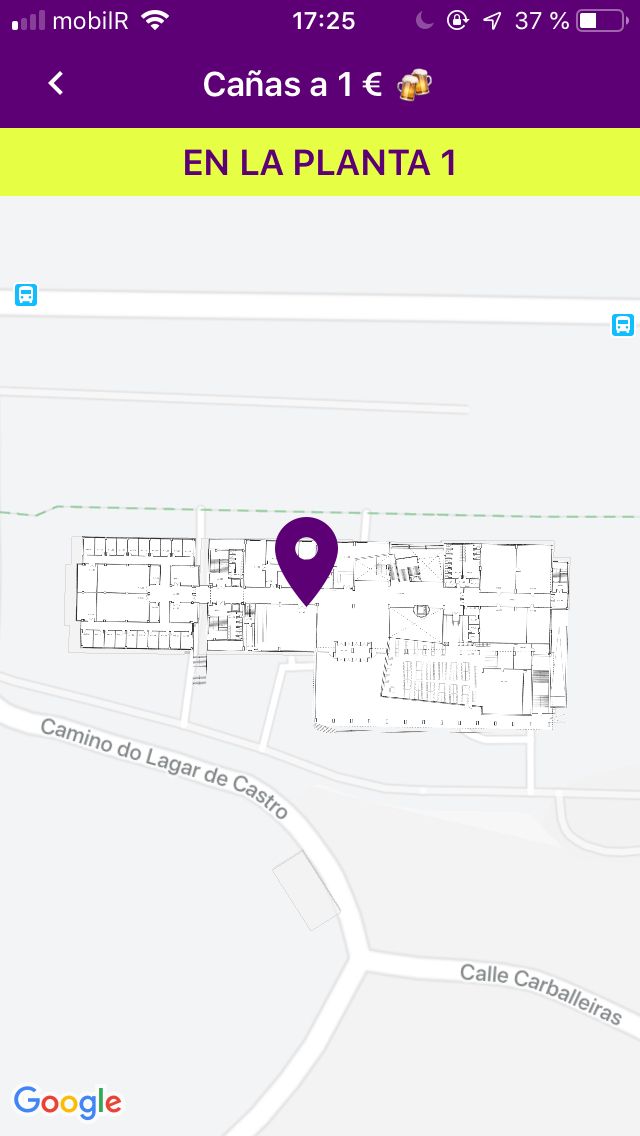
\includegraphics[scale=0.2]{figures/map-detail.jpeg}\label{fig:map-detail}}
\caption{Detalle oferta: (a) Oferta en detalle para un usuario sin autenticar/autenticado y (b) mapa que muestra únicamente una oferta.}
\end{figure}

\subsection{Mapas}
Aquí hablaremos sobre las pantallas que contienen mapas, en la aplicación nos encontramos con varias, que a pesar de ser parecidas, tienen propósitos diferentes.

\paragraph{Mapa completo del edificio.} Aquí el usuario puede explorar el edificio, seleccionando la planta que le interesa. También podrá ver la situación de todas las ofertas que no haya rechazado previamente y acceder al detalle de las mismas seleccionando el marcador en el mapa. Si se encuentra en el centro comercial, podrá ver también su posición con exactitud, ver subfigura~\ref{fig:building-map}.

\begin{figure}[tbp]
\centering
\subfigure{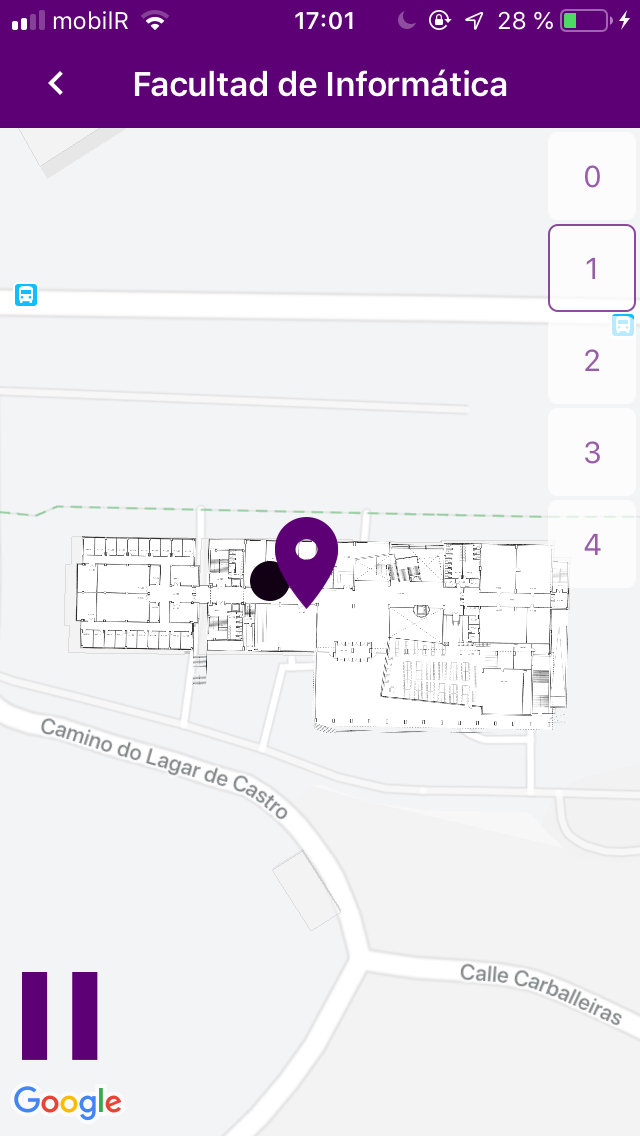
\includegraphics[scale=0.2]{figures/building-map.jpeg}\label{fig:building-map}}
\subfigure{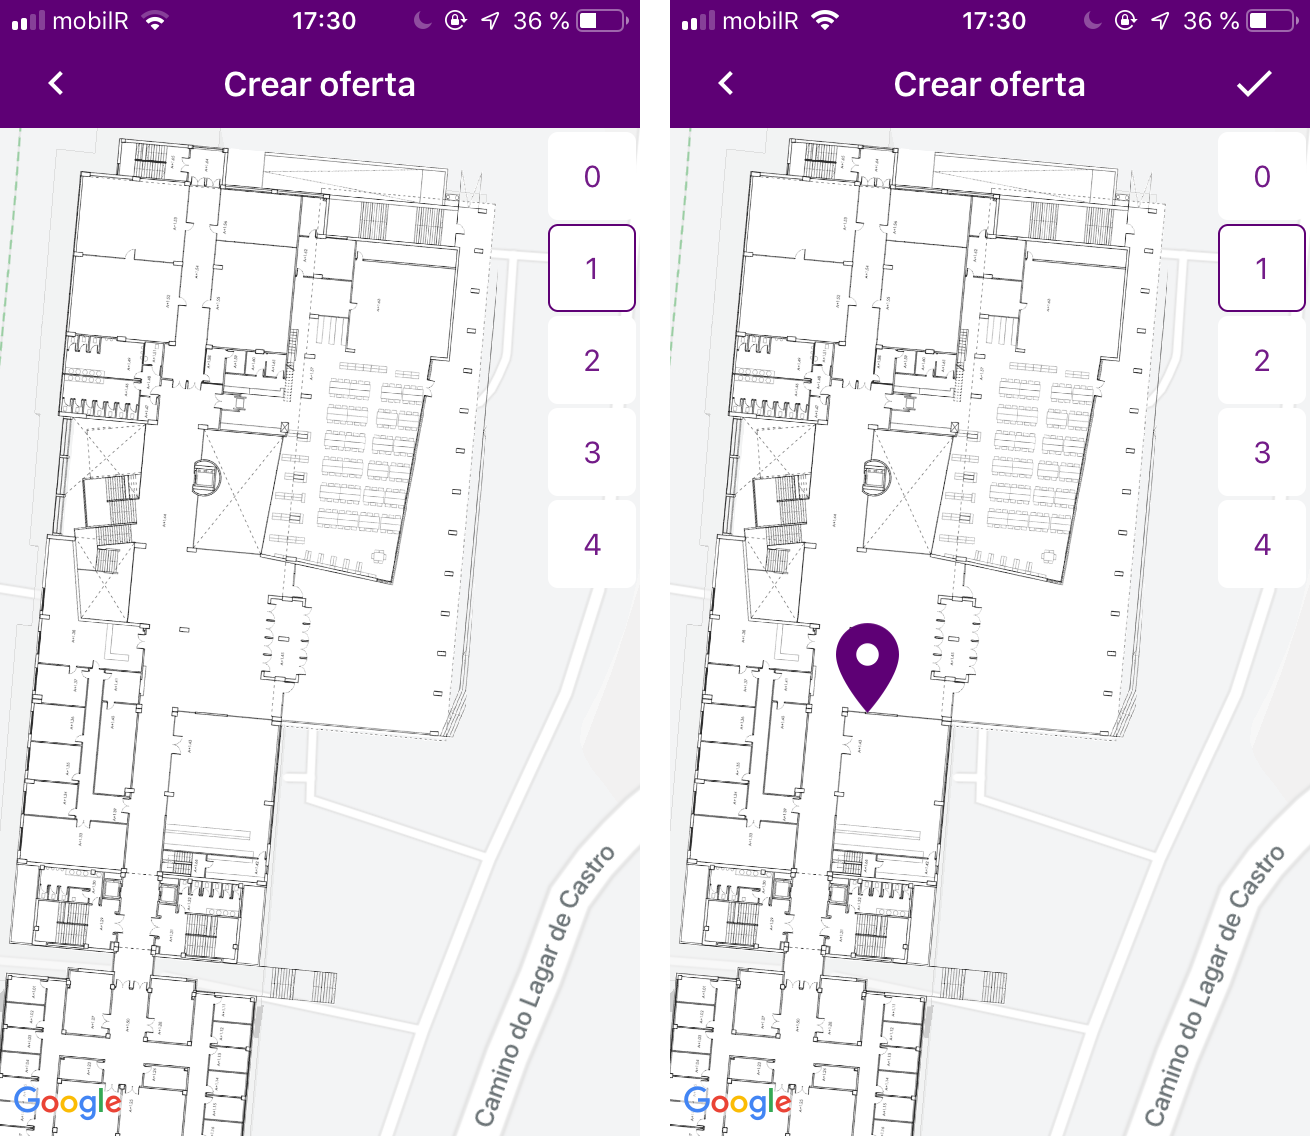
\includegraphics[scale=0.2]{figures/map-newoffer.png}\label{fig:newoffer}}
\caption{Mapas: (a) Mapa completo del edificio (aparece el icono de pausa porque es una simulación) y (b) marcar en el mapa la posición de la nueva oferta.}
\end{figure}

\paragraph{Situación de una oferta concreta en el mapa.} A partir del detalle de una oferta podemos ver su posición en el mapa. Se indicará la planta en la que se encuentra y no se podrá seleccionar otra, ver subfigura~\ref{fig:map-detail}.

\paragraph{Creación de una nueva oferta.} Cuando un usuario con rol de \textit{Propietario de tienda} quiere crear una nueva oferta, tiene que seleccionar la ubicación de la misma en el plano del centro comercial, ver subfigura~\ref{fig:newoffer}.

\subsection{Pantalla de perfil}
Si el usuario está autenticado, podrá ver las ofertas recibidas, las favoritas, las que no le interesan y las que ha canjeado. Estas funciones están deshabilitadas para usuarios que no han iniciado sesió. Además de las ofertas del usuario, en la pantalla de perfil se mostrarán ajustes relativos a las notificaciones, los cuales están disponibles para cualquier tipo de usuario, ver subfigura~\ref{fig:notif}. También encontraremos en esta pantalla, un botón que abrirá el escáner de códigos QR, para que los empleados puedan cajear ofertas, ver subfigura~\ref{fig:no-auth-qr}.

\begin{figure}[tbp]
\centering
\subfigure{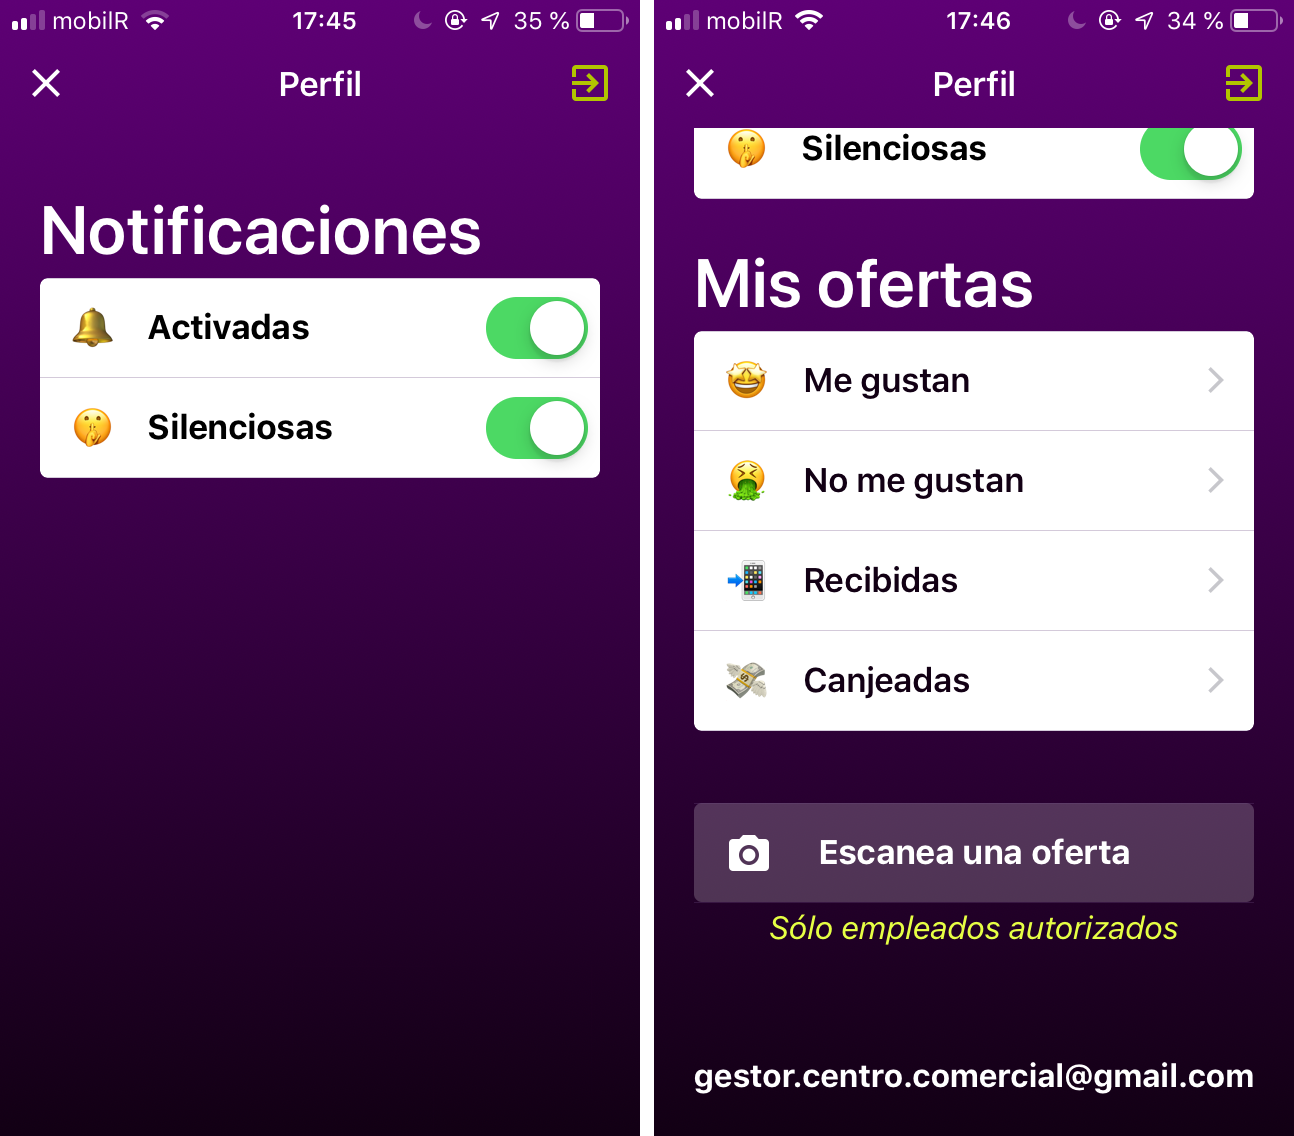
\includegraphics[scale=0.2]{figures/perfil.png}\label{fig:notif}}
\subfigure{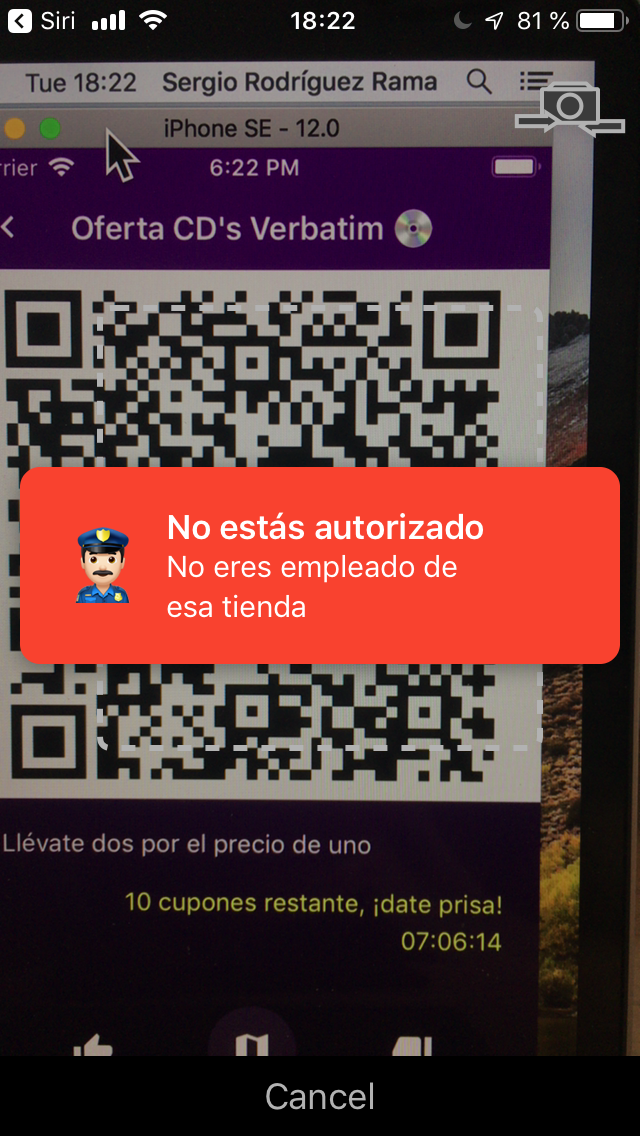
\includegraphics[scale=0.2]{figures/no-auth-qr.PNG}\label{fig:no-auth-qr}}
\caption{Perfil: (a) Usuario no autenticado vs usuario autenticado y (b) escáner con alerta informando al empleado de que no está autorizado para canjear esa oferta.}
\end{figure}

\paragraph{Ofertas favoritas o \textit{likes}.} Son aquellas ofertas en las que hemos pulsado el botón de \textit{like}. El usuario siempre tiene la opción de eliminar una oferta de favoritas o de indicar que ya no le gusta, ver figura~\ref{fig:megustan}.

\begin{figure}[tbp]
\centering
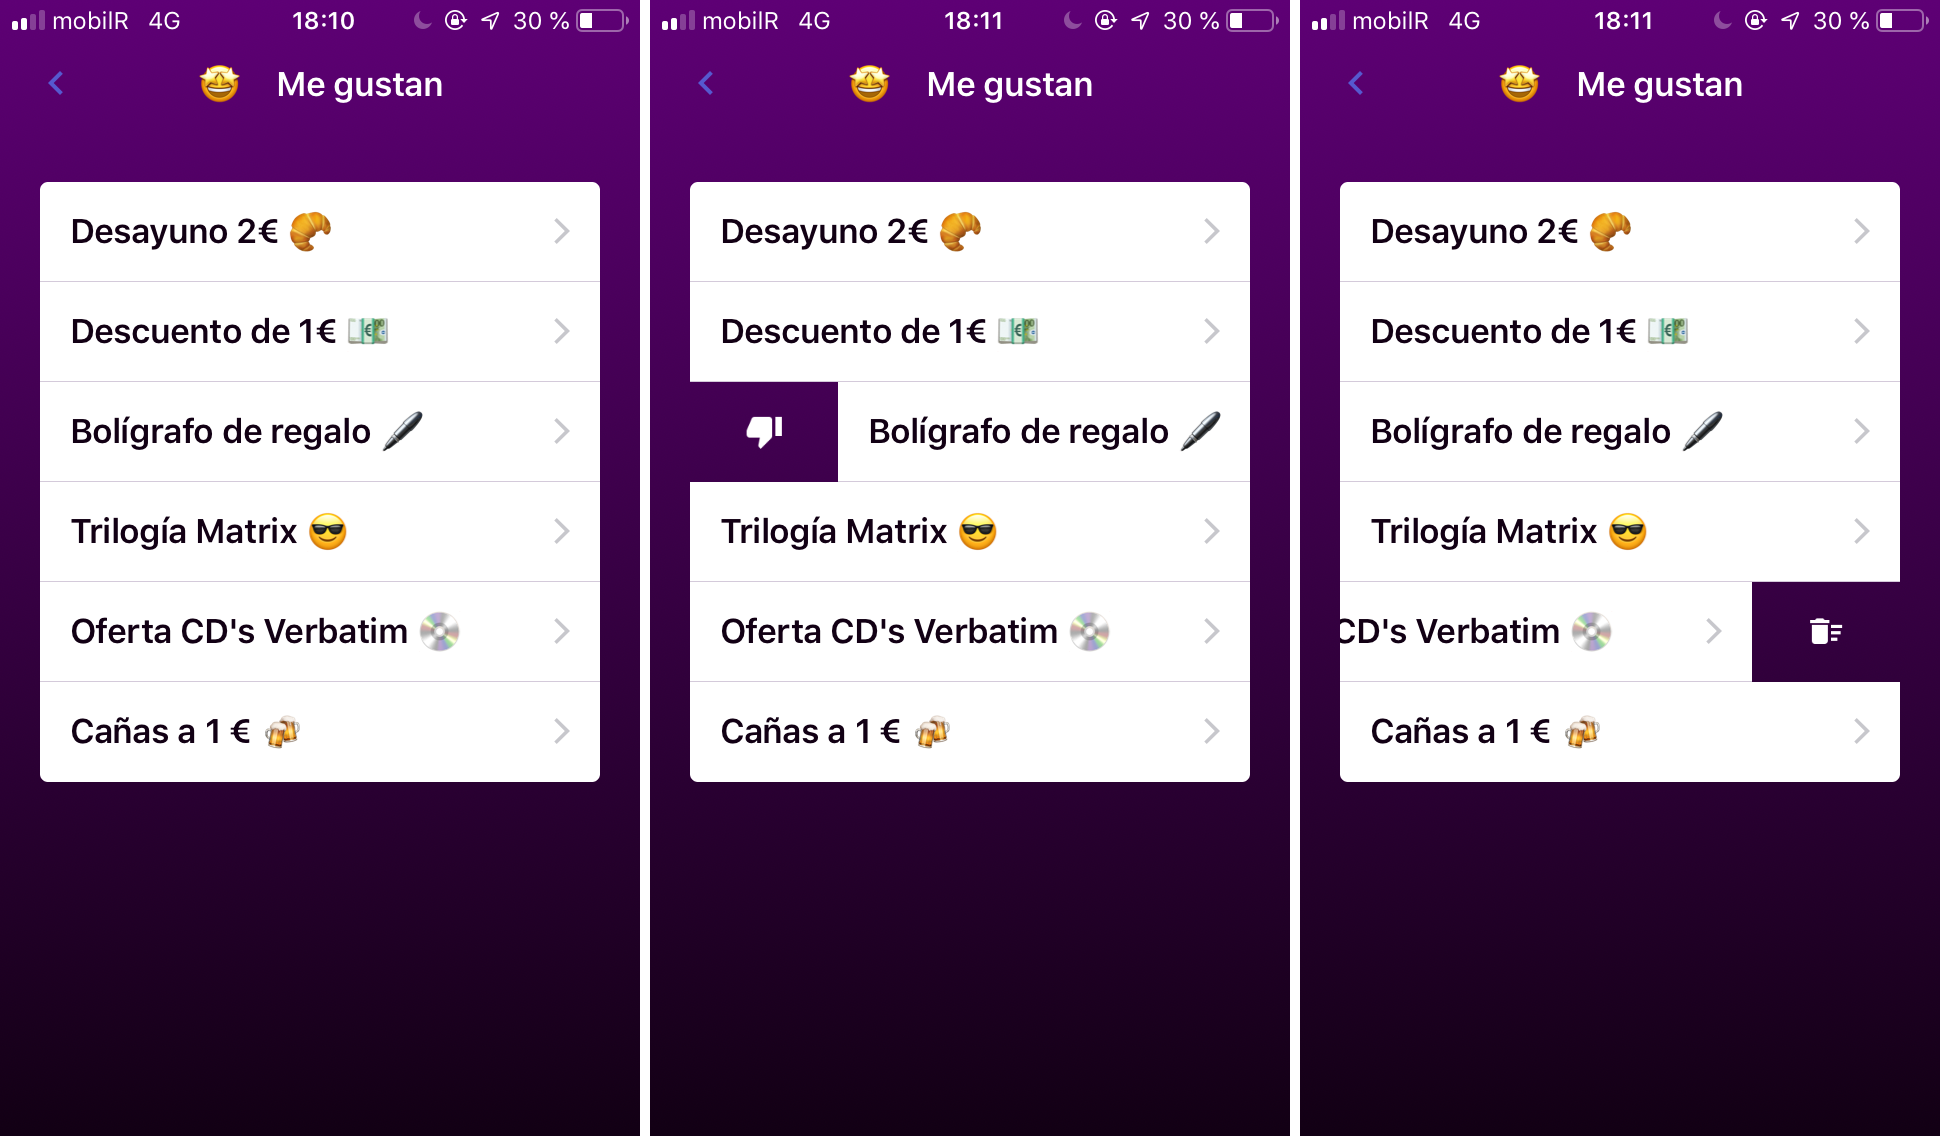
\includegraphics[scale=0.2]{figures/megustan.png}
\caption{Ofertas favoritas del usuario, deslizando la celda aparecen las opciones de borrar o de mover a rechazadas.\label{fig:megustan}}
\end{figure}

\paragraph{Ofertas rechazadas o \textit{dislikes}.} Son aquellas ofertas en las que hemos pulsado el botón de \textit{dislike}. El usuario siempre tiene la opción de eliminar una oferta de rechazadas o de indicar que ha cambiado de opinión y que ha decidido que le gusta. La pantalla sería exactamente igual que la de los \textit{likes} (figura~\ref{fig:megustan}), simplemente se cambiaría el botón de \textit{dislike} por el de \textit{like}.

\paragraph{Ofertas recibidas.\label{item:recibidas}} Estas son las ofertas con las que se ha cruzado el usuario. Se lleva un registro de las mismas, por si acaso no tenía activadas las notificaciones o no estaba atento a la aplicación cuando se las cruzó. De esta manera, puede llegar a casa y revisarlas para indicar cuales le gustan y cuales no, o simplemente ignorarlas. Cuando un usuario indica que una de estas ofertas le gusta o no, desaparece del listado de ofertas recibidas y pasa a favoritas o rechazadas, ver figura~\ref{fig:recibidas}.

\begin{figure}[tbp]
\centering
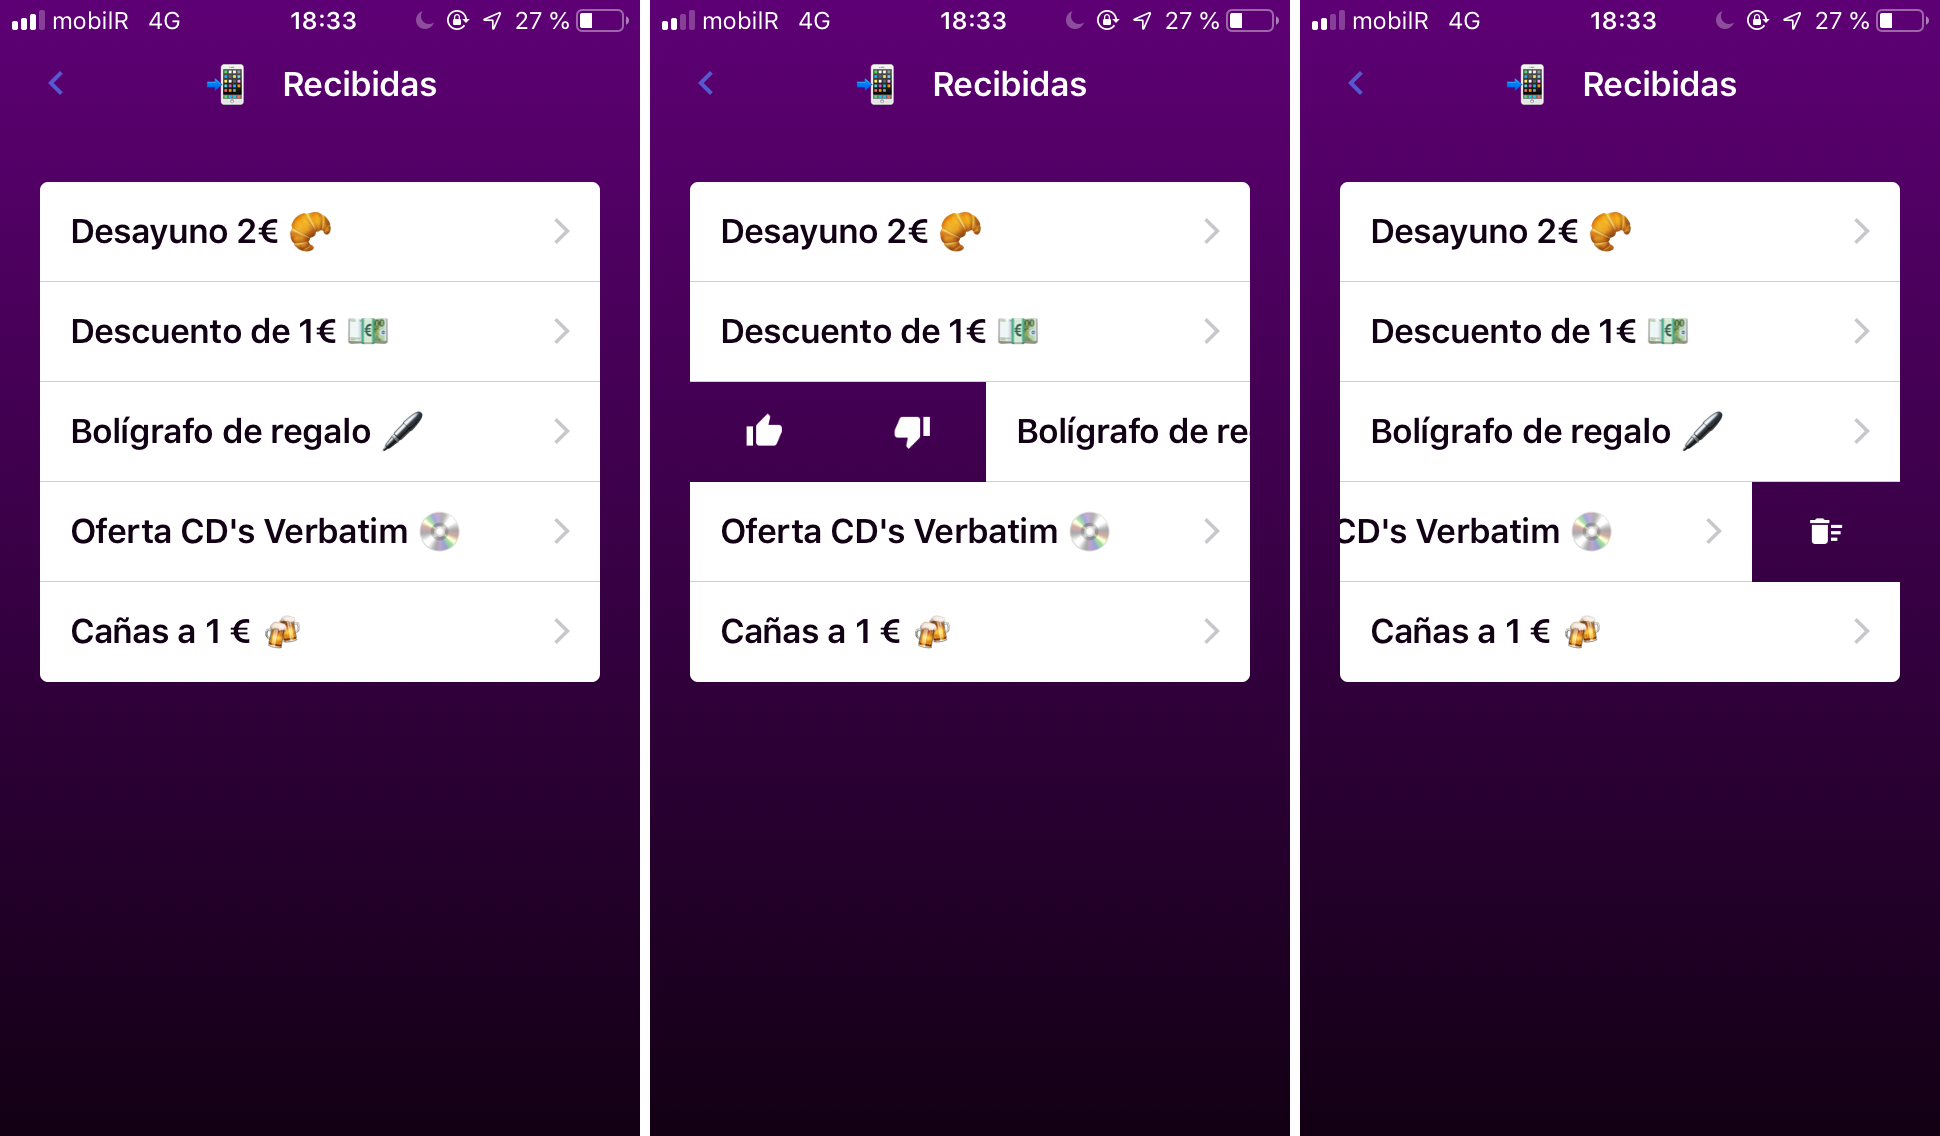
\includegraphics[scale=0.2]{figures/recibidas.png}
\caption{Ofertas recibidas, deslizando la celda aparecen las opciones de borrar o de \textit{like}/\textit{dislike}.\label{fig:recibidas}}
\end{figure}

\paragraph{Ofertas canjeadas.} Estas son las ofertas que el usuario ha canjeado. Se lleva un registro de las mismas por motivos de seguridad, en caso de que el usuario quiera reclamar algo se podrá ver con facilidad si ya ha disfrutado la oferta o no. Esta pantalla es exactamente igual que las anteriormente comentadas (figura~\ref{fig:recibidas} y figura~\ref{fig:megustan}), con la diferencia de que al deslizar la celda no encontramos ningún botón ni de me gusta/no me gusta, ni de eliminar. Ya que no se quiere que las ofertas desaparezcan de ahí.

\subsection{Roles}
Hasta ahora hemos visto la aplicación como la vería un usuario normal, autenticado o sin autenticar, salvo por la subfigura~\ref{fig:newoffer} que corresponde a una pantalla que sólo los propietarios de las tiendas podrán ver. A continuación, veremos como se han distribuido las acciones propias de los otros cuatro roles.

\paragraph{Administrador de la plataforma.} Cuando el administrador de la plataforma selecciona un centro comercial, se le ofrece la posibilidad de añadir un nuevo gestor. La pantalla de añadir un nuevo rol es igual para gestores, propietarios y empleados \ref{addrol}.

\paragraph{Gestor de un centro comercial.} Cuando un usuario es nombrado gestor de un centro comercial, en su pantalla aparece en tiempo real un botón que le permite añadir una nueva tienda, llevándolo a otra muy similar a la de añadir rol en la que simplemente le pregunta el nombre del establecimiento. Y si está en la pantalla correspondiente a una tienda, aparecerá un botón que le permitirá añadir un propietario a la misma, ver figura~\ref{addrol}.

\begin{figure}[tbp]
\centering
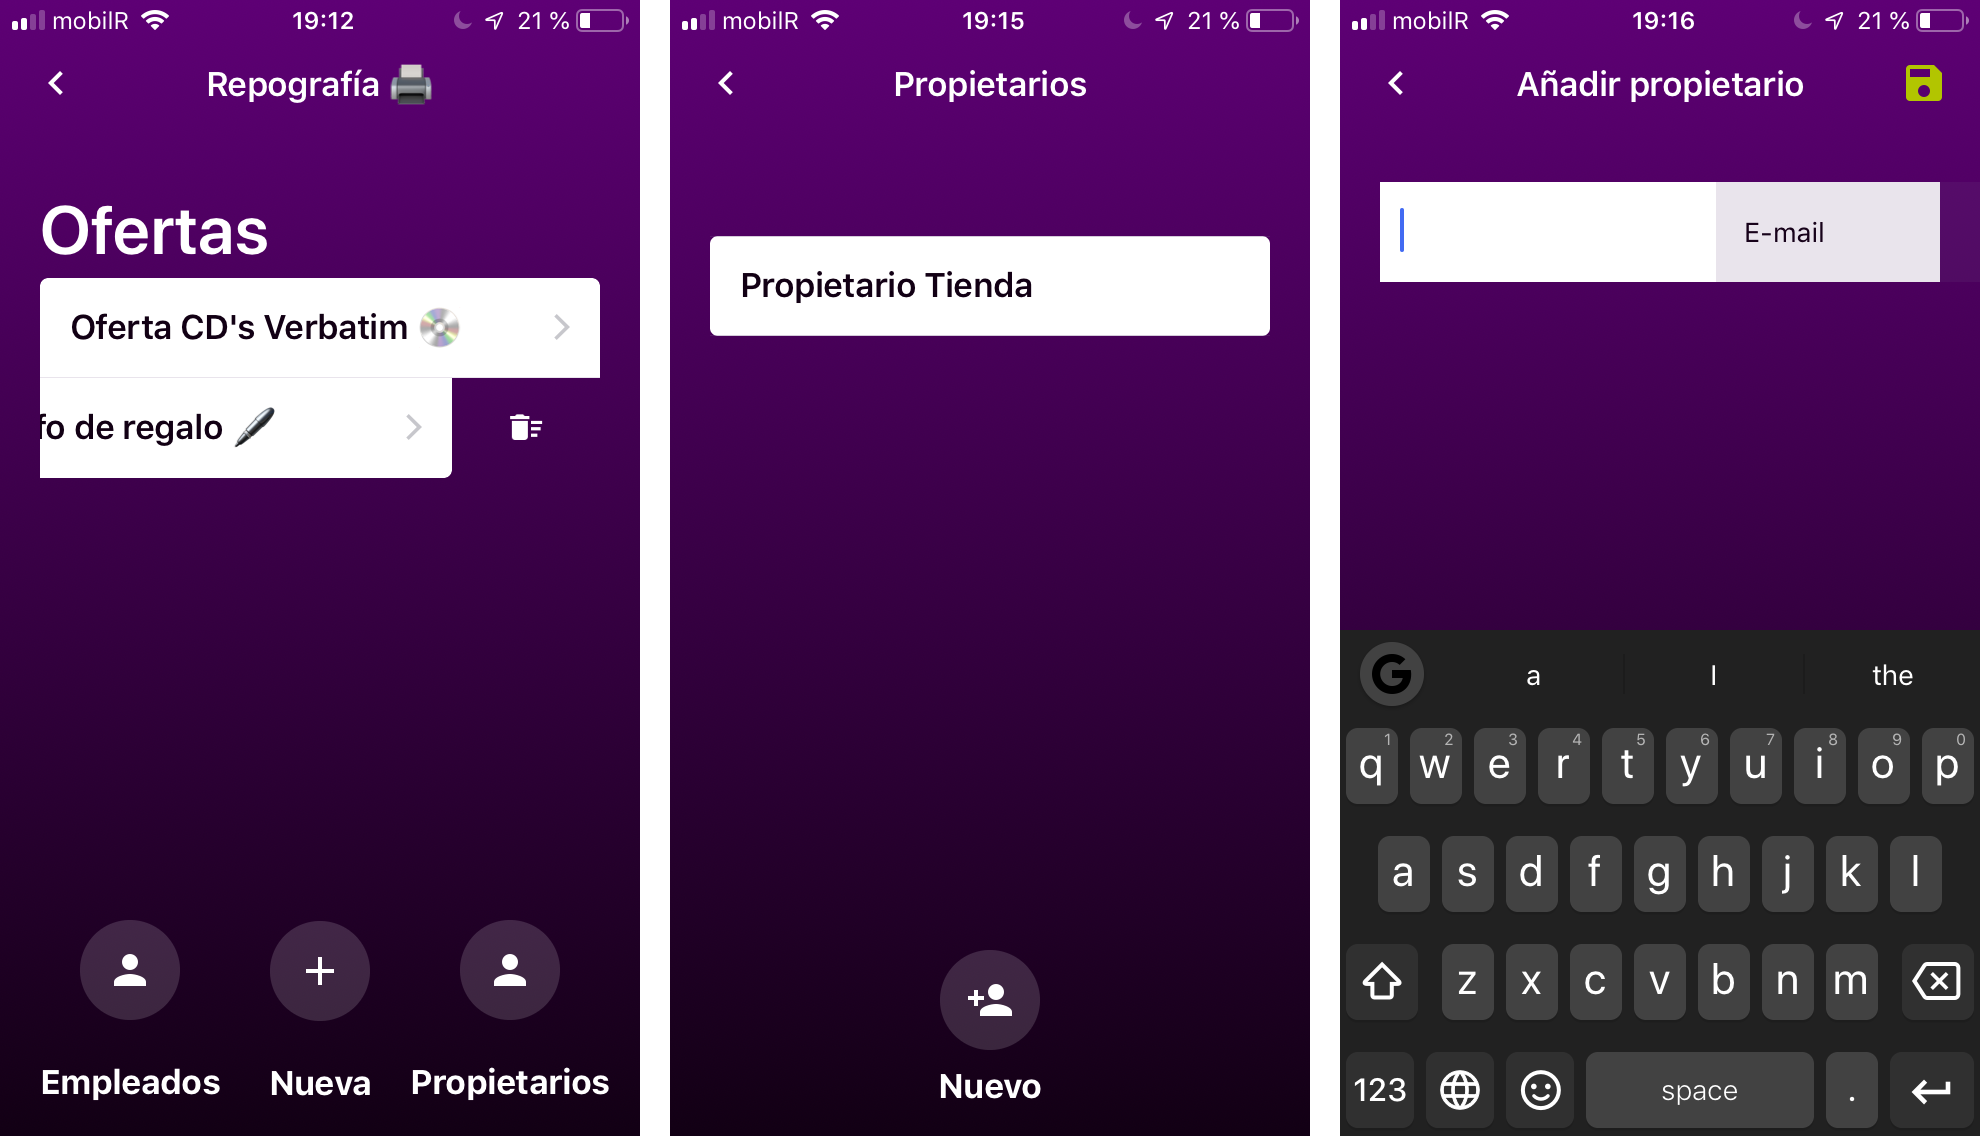
\includegraphics[scale=0.2]{figures/anadir-rol.png}
\caption{Estas capturas fueron tomadas con la aplicación en modo desarrollo con todas las funcionalidades desbloqueadas, por eso aparecen los botones de \textit{Empleados} y \textit{Propietarios}, dos acciones que corresponden a roles diferentes y que no deberían aparecer en la misma pantalla.\label{addrol}}
\end{figure}

\paragraph{Propietario de una tienda.} Cuando un usuario es nombrado propietario de una tienda, aparecerá en su pantalla la posibilidad de añadir un empleado o una oferta a la misma. Para añadir una oferta, primero hay que marcar su posición en el plano, como en la subfigura~\ref{fig:newoffer} y a continuación, darle un nombre, una descripción, el radio de acción, la duración y el número de unidades disponibles, ver figura~\ref{fig:newoffer2}.

\begin{figure}[tbp]
\centering
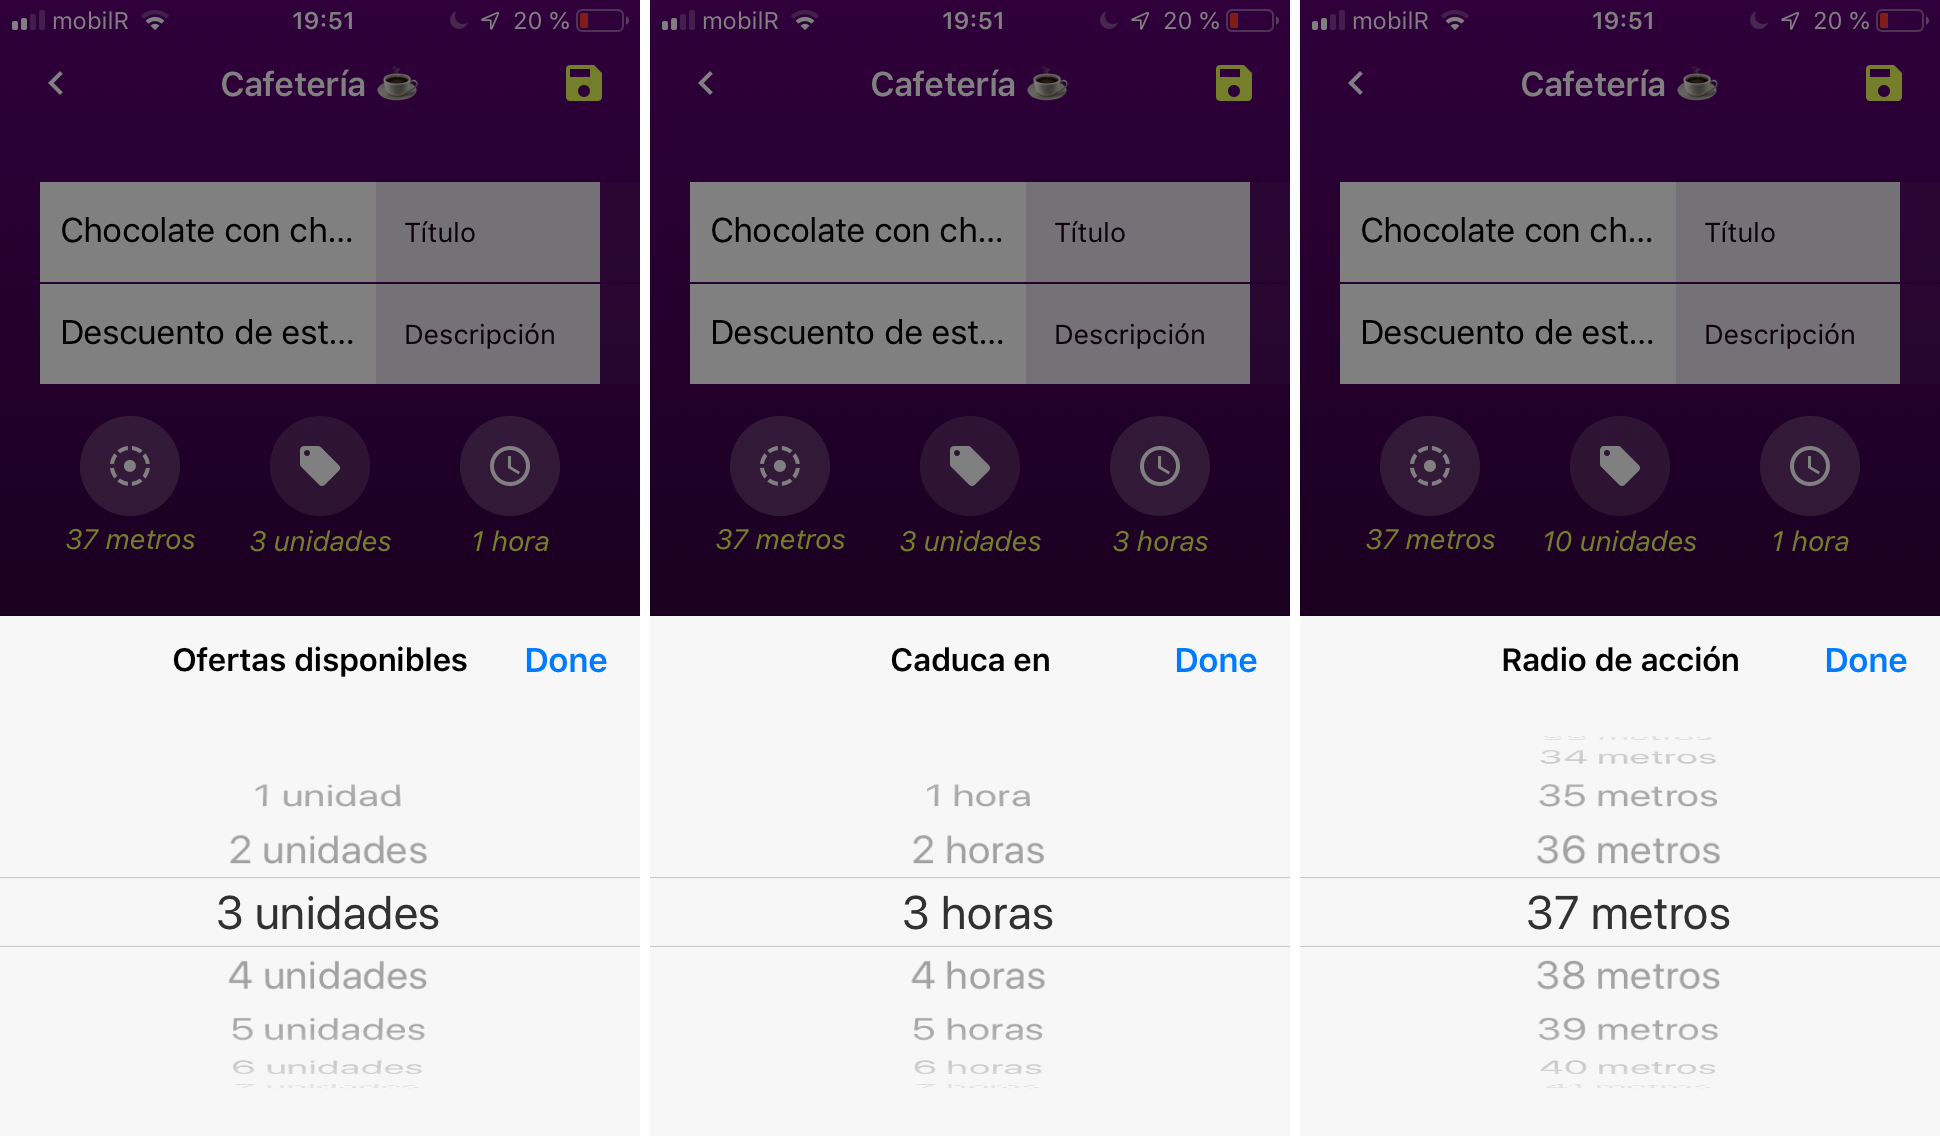
\includegraphics[scale=0.2]{figures/newoffer2.png}
\caption{Cuando el propietario selecciona alguno de los botones de radio de acción, duración o unidades; se muestra un selector.\label{fig:newoffer2}}
\end{figure}

\paragraph{Empleado de una tienda.} Cuando un usuario es nombrado empleado de una tienda, podrá empezar a canjear ofertas de la misma. Se hablará más a fondo sobre esto, más adelante \ref{qr}.


\subsection{Notificaciones}
Cuando un cliente va caminando por un centro comercial, irá recibiendo notificaciones cada vez que entra en el rango de acción de una oferta, ver figura~\ref{fig:notificacion}. Puede tenerlas bloqueadas, en este caso no recibirá ninguna notificación; o silenciadas para que aparezcan las notificaciones pero no emitan ningún sonido \ref{fig:notif}. 

\begin{figure}[tbp]
\centering
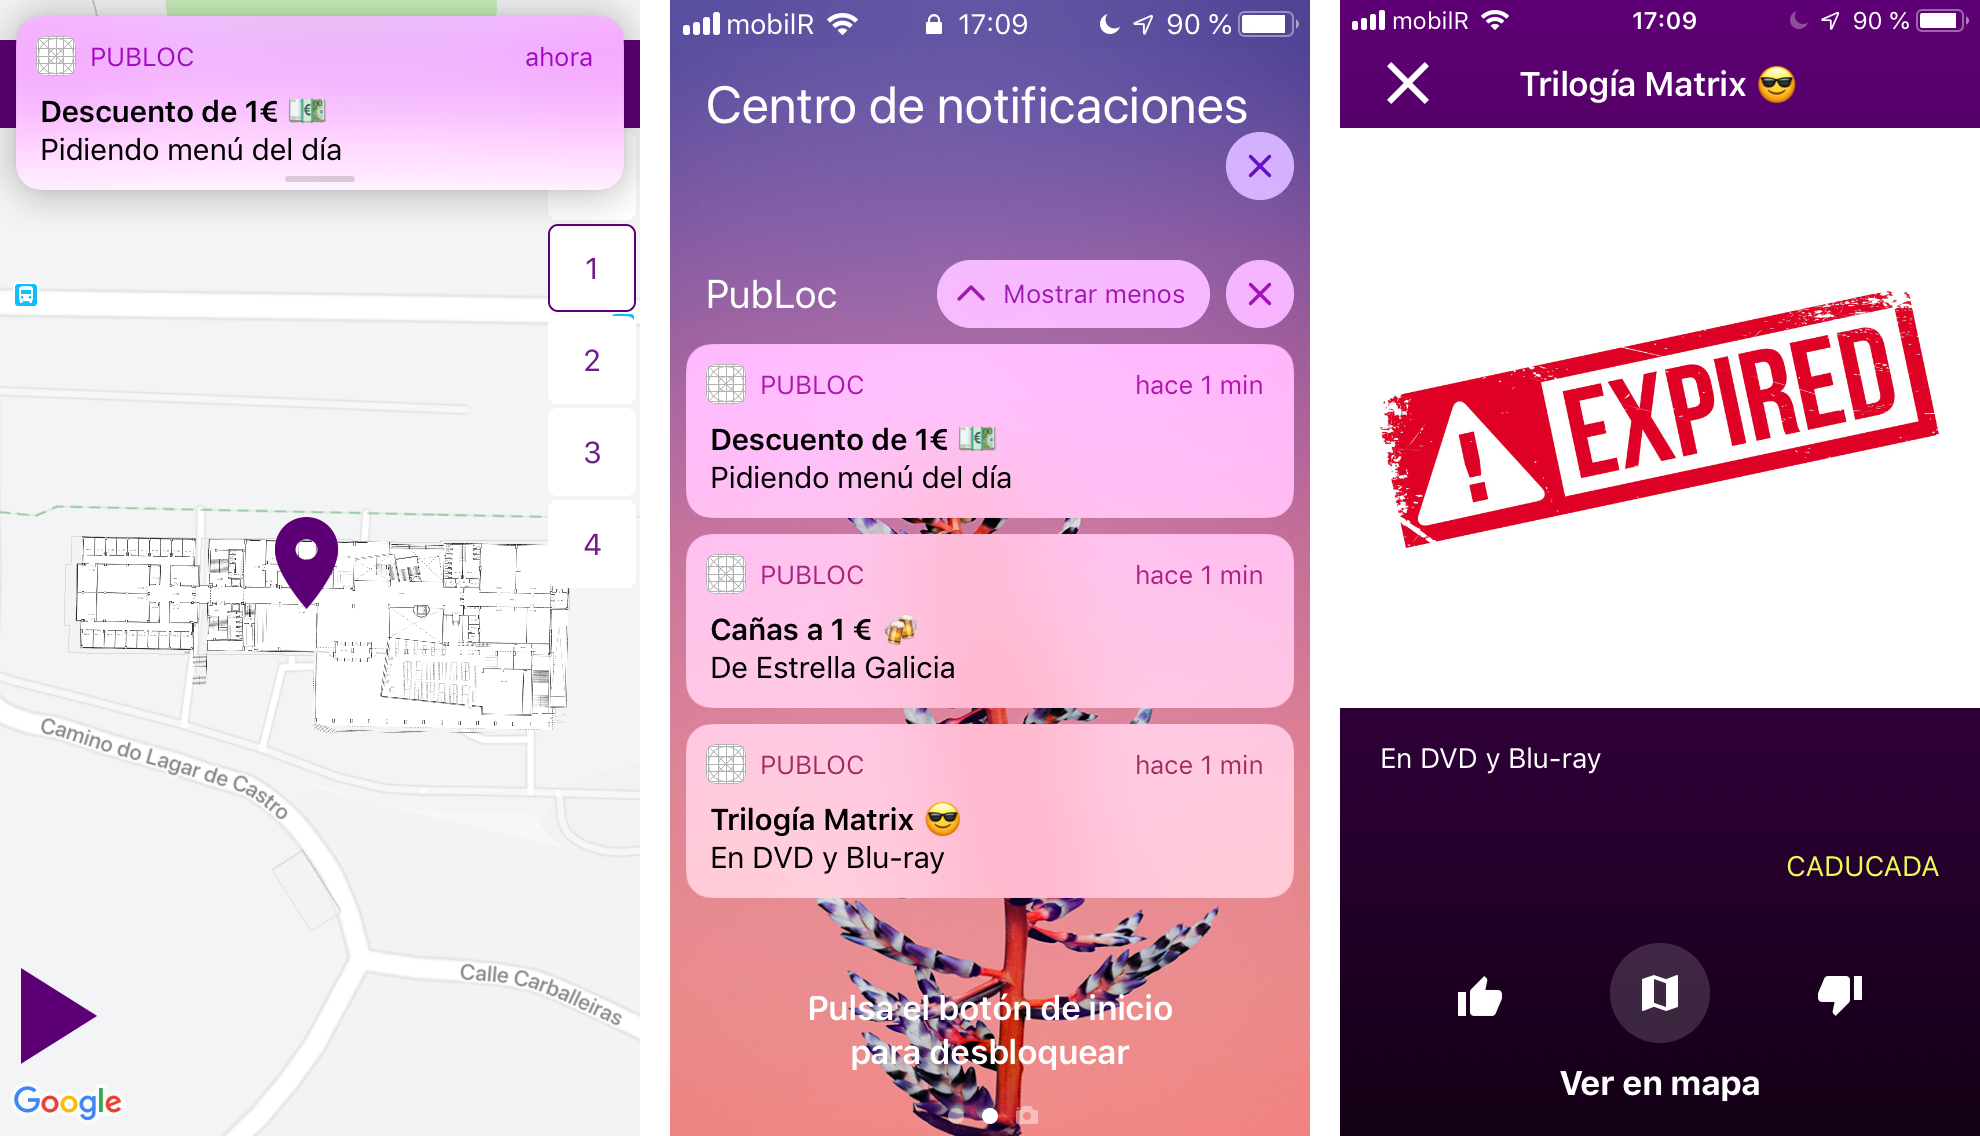
\includegraphics[scale=0.2]{figures/notificacion.png}
\caption{Ciclo de vida de una notificación.\label{fig:notificacion}}
\end{figure}

Estas notificaciones se almacenarán en el centro de notificaciones aunque tengamos el teléfono bloqueado, para así poder consultarlas más tarde. Como ya se comentó más arriba \ref{item:recibidas}, en caso de que se tengan las notificaciones desactivadas, siempre se podrán revisar las ofertas que se han recibido.



\subsection{\textit{Siri} y escaneo de códigos \textit{QR}} \label{qr}
Una de las funciones más atractivas de la aplicación es la de escanear códigos QR para canjear ofertas. Cuando un cliente llega con su código \textit{QR} al mostrador, el empleado de esa tienda podrá canjearla si no está caducada, quedan unidades o el usuario no la ha disfrutado ya. Hay dos maneras mediante las cuales un empleado puede acceder al escáner de códigos \textit{QR}.

\paragraph{A través de su perfil.} Hay un botón en esta pantalla que permite acceder a esta funcionalidad, ver subfigura~\ref{fig:notif}.

\paragraph{Atajos de \textit{Siri}.} Con \textit{iOS 12}, que en la fecha en la que se desarrolló la aplicación todavía estaba en estado beta, nace la posibilidad de vincular funciones de nuestra aplicación con comandos de voz que nosotros mismos podemos configurar a nuestro gusto (figura~\ref{fig:siri}), llamados \textit{Atajos de Siri}.

\begin{figure}[tbp]
\centering
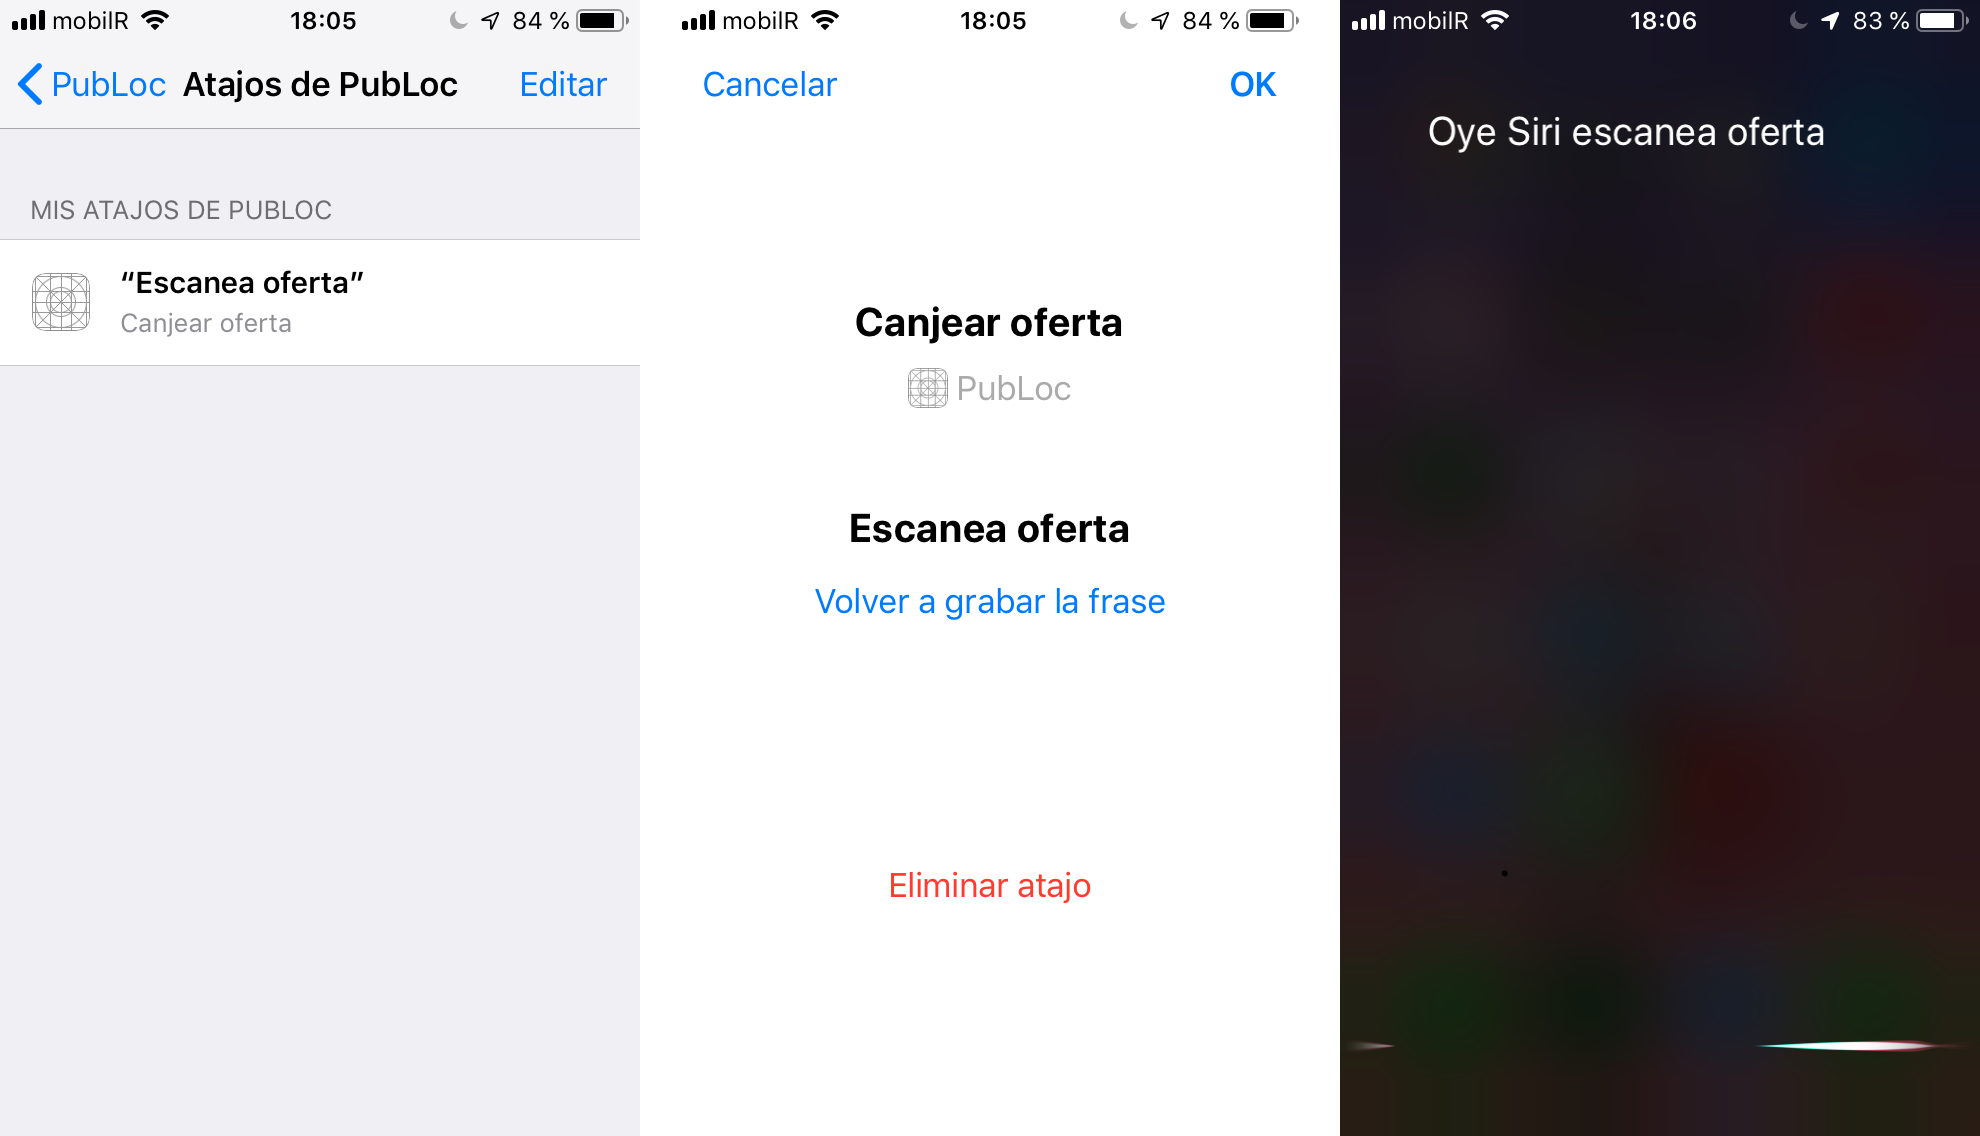
\includegraphics[scale=0.2]{figures/siri.png}
\caption{Creación de un atajo de \textit{Siri}.\label{fig:siri}}
\end{figure}

Una vez canjeada la oferta, tanto el cliente como el empleado deben recibir una confirmación visual. En el móvil del empleado aparece una alerta que le indica que ha concluido el escaneo y el móvil del cliente, el código \textit{QR} se cambia por otra imagen que le indica que ya ha canjeado la oferta, ver subfigura~\ref{subfig:exito-qr}.

\subsubsection{Errores de escaneo}
Puede ser que un escaneo no pueda realizarse, bien por una mala lectura o un código \textit{QR} incorrecto o por otro tipo de situaciones.

\paragraph{El empleado no está autorizado para escanear esa oferta.} Esto sucede porque el usuario que la escanea no trabaja en la tienda a la que pertenece.

\paragraph{Oferta ya canjeada por ese usuario.} Cabe la posibilidad de que un usuario canjee la misma oferta más de una vez. Puede pasar sin querer, porque tiene en modo avión el teléfono y no se marca como canjeada, por ejemplo. Pero también puede hacerlo a propósito, sacando una captura de pantalla antes de canjearla e intentando canjearla de nuevo más tarde. Para evitar estas situaciones, se comprueba que el usuario no haya disfrutado la oferta con anterioridad, ver subfigura~\ref{subfig:trampa-qr}.

\begin{figure}[H]
\centering
\subfigure{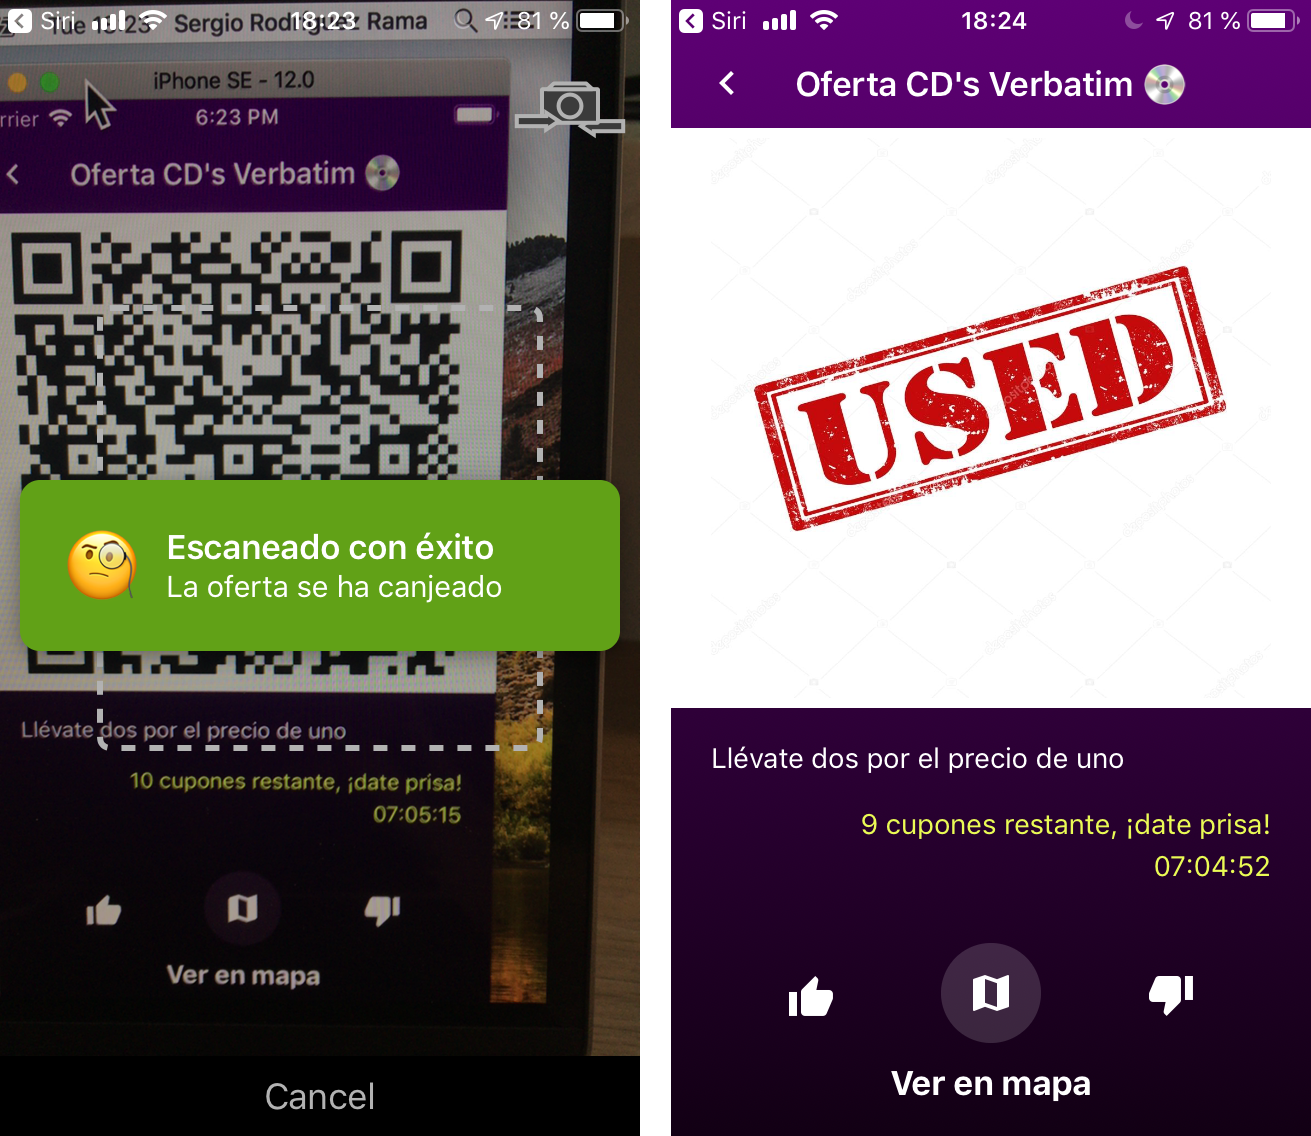
\includegraphics[scale=0.2]{figures/exito-qr.png}\label{subfig:exito-qr}}
\subfigure{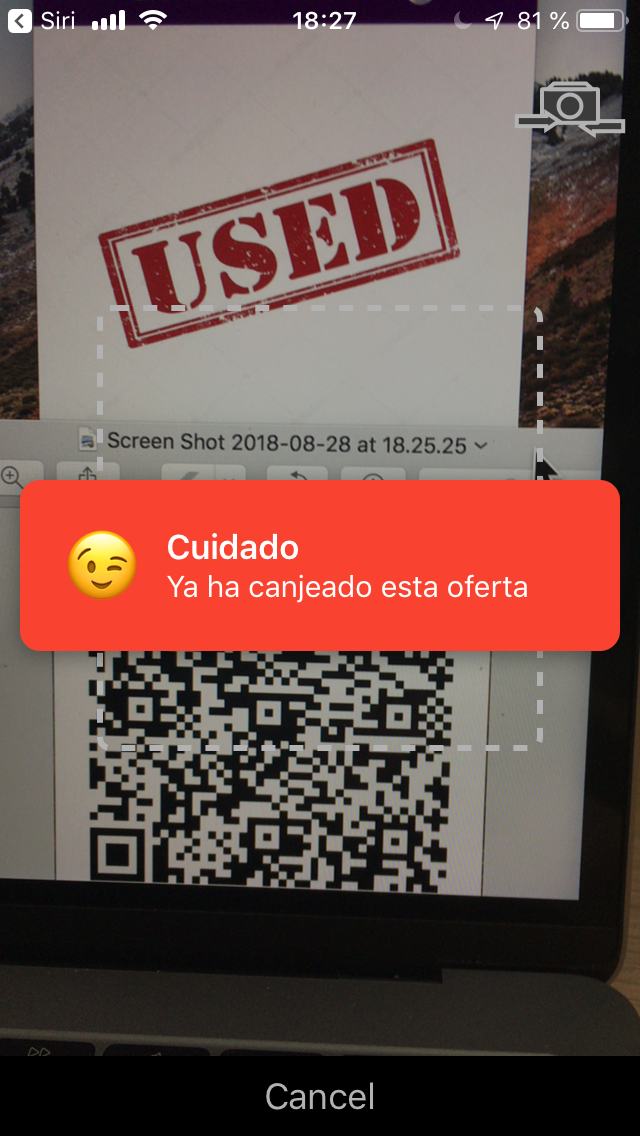
\includegraphics[scale=0.2]{figures/trampa-qr.PNG}\label{subfig:trampa-qr}}
\caption{Escáner \textit{QR}: (a) Confirmación de escaneo en móvil del empleado y del cliente y (b) ejemplo de lo que pasaría si un cliente tratase de hacer trampas con una captura de pantalla.}
\end{figure}
